\pdfoutput=1

\documentclass[11pt]{article}

\usepackage{wiki-savvy-rag}
\usepackage{times}
\usepackage{latexsym}
\usepackage[T1]{fontenc}
\usepackage[utf8]{inputenc}
\usepackage{microtype}
\usepackage{inconsolata}
\usepackage{natbib} % this is probably into you nips_2018 format file
\usepackage{graphicx}
\usepackage{geometry}
\usepackage{subcaption}


\newcommand{\sideBySideImages}[5]{%
    \begin{figure}[ht]
        \centering
        \begin{subfigure}{#3\linewidth}
            \centering
            \includegraphics[width=\linewidth]{#1}
        \end{subfigure}%
        \hfill%
        \begin{subfigure}{#3\linewidth}
            \centering
            \includegraphics[width=\linewidth]{#2}
        \end{subfigure}
        \caption{#5}
        \label{#4}
    \end{figure}
}

% TODOS:
% - Add the MMLU results and figures
% - In the abstract, briefly mention our findings once we have some
% - rewrite the conclusion
% embeddings section: first one to go in need of space


% findings:
% - accuracy during training ?


\title{Wikipedia-Savvy-RAG: Wikipedia-backed RAG system expert about STEM subjects}  

\author{Dario Filatrella \and Michele Palma \and Mattia Scardecchia \and Federico Zarantonello}

\begin{document}
\maketitle
\begin{abstract}
We present Wikipedia-Savvy-RAG, a lightweight Retrieval-Augmented Generation (RAG) system for
STEM domain question answering. To improve performance in knowledge intensive tasks we filtered, cleaned, 
chunked and embedded the English Wikipedia and built a vector database of STEM-focused semantic embeddings. 
Then, we used QLORA to efficiently finetune a small pretrained language model 
(500M params) on a subset of the Yahoo Answers dataset, feeding the model with the most relevant passages from the 
vector database and keeping the query and passage embedders frozen. Finally, we used the MMLU dataset to 
benchmark our system and run a variety of ablation studies, using the pretrained llm without RAG as our baseline.
We show that even a small LLM can benefit from retrieval, and that [TODO: fill!].
The system is lightweight and can be deployed on most modern personal computers. To demonstrate its capabilities,
we developed a Streamlit web application that allows users to interact with the model in real-time with a chat-like interface.
Experiments are fully reproducible and the code is available at \url{https://github.com/spring-projects-2024/wiki-savvy-rag}.

\end{abstract}

\section{Introduction and Related Works}

In recent years, the field of natural language processing has seen a surge in
the development of large language models (LLMs) that can generate human-like text. \cite{gpt3}
These models have been used in a variety of applications, such as chatbots,
question-answering systems, and text summarization, with remarkable performance.  \cite{nlp_applications}
However, LLMs often struggle with generating accurate and informative responses, especially in specialized
domains like science, technology, engineering, and mathematics (STEM).  \cite{hallucinations_llm}

A successful approach to address this limitation has been the combination of LLMs with retrieval
mechanisms from a knowledge base to generate more accurate and informative responses.
Along this line of research, started with \cite{rag_paper}, several variants and improvements have been proposed,
such as \cite{replug} \cite{radit}. These are extensively reviewed in \cite{rag_survey}.

In this paper, we present Wikipedia-Savvy-RAG, a lightweight RAG system fine-tuned for STEM question answering
in chat format. In building our system, we strived to keep the computational resources required for both
training and inference contained. Indeed, our system can be deployed on personal computers with a CUDA-enabled GPU
with at least 8GB of memory, through a Streamlit web application we developed. Furthermore, the finetuning can 
be replicated on a single consumer-grade GPU in a few hours. In doing so, the main research question that we aimed to
answer is whether and to what extent a small LLM can benefit from retrieval in knowledge intensive tasks, and whether a
simple finetuning recipe under tight computational constraints can still improve performance. 

To build the vector database, we processed the English Wikipedia available on WikiMedia \cite{wikimedia} and obtained 
dense representations of the chunks using a lightweight text embedder \cite{baai}. We then built a vector database using
the Faiss library \cite{faiss} and SQLite \cite{sqlite} to index and retrieve embeddings and passages, respectively. To keep resources low,
we employed a small pretrained LLM with 500M parameters \cite{qwen}, and we used QLORA \cite{qlora} to finetune it efficiently, 
keeping the embedder frozen, on a subset of the Yahoo Answers dataset \cite{yahoo_answers}.
In order to benchmark our system and conduct a variety of ablation studies, we used the MMLU dataset \cite{mmlu}.

This report will outline the steps we took to build our system, the motivations behind our choices, and the results of our evaluation.
We will also discuss potential improvements and future work.

\section{Knowledge Base}

Since we decided to focus on STEM subjects, we needed a knowledge base that was rich in scientific and technical information.
We downloaded the English Wikipedia dump, filtered the articles related to STEM subjects, and cleaned the text.

\subsection{Filtering and Cleaning}

We downloaded the dump dated 20 December 2023 (100GB) from WikiMedia \cite{wikimedia}. Wikipedia articles have category tags to help classify them.
Categories are organized in a directed acyclic graph (DAG), but not a tree \cite{wikipedia_category_tree}. To keep STEM articles, we marked only the categories that are at
distance at most k from a set of hand-picked root categories in the category DAG, and we kept articles belonging to the marked categories.
Then, we used regular expressions and many Python scripts to remove (almost) everything that wasn't plain text, such as XML tags, tables, and references. After filtering, the XML
dump was reduced to 22GB. After cleaning, it went down to 8GB.

Then we proceeded in splitting the articles into the different sections to obtain the chunks 
that will be used by the RAG model. 
In the end we obtained a total of 13 million chunks, with an average length of about 230 words.
We stored all of these, together with their titles, in an SQLite database.

\subsection{Embeddings}

We tokenized and embedded the chunks using the open-source BAAI/bge-small-en-v1.5 model 
\cite{bge_hf}. This model is the smaller version of the BAAI General Embeedding family v1.5. 
To get the dense embeddings for sentences, it uses the last hidden state of the [CLS] token, and it outputs 
384-dimensional vectors.

We chose this model for its balance between performance and computational cost.
In fact, the embedder is significantly smaller than its peers, being a BERT-like model with 33.4M 
parameters and only 0.12GB of memory usage, but achieves a 51.68 score on the MTEB Retrieval task.

\subsection{Vector Database}

We used the Faiss library to build a vector database of the embeddings for efficient retrieval, using dot product to compare vectors.
Faiss is a library for efficient similarity search and clustering of dense vectors that offers different indexing methods.
We mostly investigated three index variants: Flat uses simple brute-force search, IVF uses centroid-based clustering to 
implement a hierarchical search that reduces the number of comparisons, and HNSW creates a multi-layered graph structure 
where each layer is a simplified, navigable small world network. For further details, see the excellent Faiss documentation \cite{faiss}.

Faiss also offers different quantization techniques to reduce the memory footprint of the embeddings. We focused
on two quantization techniques: scalar quantization and product quantization. 
Scalar quantization quantizes each dimension of the vector independently in a linear
range, while the product quantization splits the vector into subvectors and quantizes each
subvector independently.

We benchmarked extensively different combinations of indexes and quantization techniques to find the best configuration
for our system. We measured recall, query time, and memory usage to find a good trade-off. See the Benchmark section for more details.
We eventually chose the Flat index with 128 subvectors product quantization.

\section{Retrieval-Augmented Generation}

\subsection{Large Language Model}

As LLM, we chose the pretrained Qwen/Qwen1.5-0.5B-Chat \cite{qwen_hf} model, the smallest model in the Qwen v1.5 family
with only 620M parameters. It was pretrained with a large amount of data, and post-trained with both supervised finetuning 
and direct preference optimization to align it with human preferences. It has a context length of 32K tokens.

\subsection{Generation}

To generate text through RAG, we need to pass retrieved passages to the model in order to produce logits
for the next token, and then use a decoding strategy to generate the final answer.
We implemented two methods to produce logits. The first one, which we refer to as 'naive', concatenates all the retrieved passages
and the query, and feeds the result to the model. The second one, following \cite{replug}, feeds the query and each individual passage
separately to the model, and then combines the predicted probabilities from each passage with weights proportional to the similarity
to get probabilities.
As for the decoding strategy, we implemented greedy decoding, top-k sampling, and top-p sampling. \cite{decoding}

\section{Finetuning}

The LLM was pretrained aligned, but it was never thought to compose its answers to user queries using retrieved passages.
To address this, we finetuned our system on a question answering task, using a simple recipe.

\subsection{Data}

As training data, we downloaded the Yahoo Answers dataset and used its metadata to filter it and keep only STEM questions. The result is around 23k
examples. As validation data, we used the validation split of the MMLU dataset \cite{mmlu_hf}. During training, for a given question, we retrieved the single most similar passage from
our knowledge base and formatted the input to meet the expectations of Qwen, including the retrieved passage as context.

\subsection{Training}

We froze the query and passage embedders and finetuned the LLM only. We used the QLORA technique \cite{qlora} to drastically reduce the number of training
parameters and the memory requirements while minimally impacting performance. In essence, this consists in freezing and quantizing the pretrained weights and adding low
rank adapters to each layer, as in \cite{lora}. Then, we backpropagate through the 4-bit quantized frozen weights to train the adapters.
As a training criterion, we use cross entropy loss between predicted logits and the ground truth answer. This allows exploiting the inherent
parallelism of the transformer architecture, since thanks to the causal mask we obtain an error signal for each ground truth token in parallel at every step.
Details about our training setup can be found in out GitHub repository.

\section{Demo}

To demonstrate the capabilities of our system, we developed a Streamlit web application
that allows users to interact with the model in real-time with a chat-like interface. 
The application lets users ask questions about STEM subjects, and the model will provide answers 
based on the Wikipedia passages it retrieves from its knowledge base. 
The user can decide the number of passages to retrieve, the decoding strategy (greedy, top-k, top-p), 
the generation type (naive or REPLUG) and other configuration parameters.
Refer to our GitHub repository for more information on the application.

\subsection{Arxiv}

A further functionality we implemented is the ability to upload Arxiv papers in Latex format and ask questions about them.
This feature is marked as experimental, as it wasn't extensively tested.

\section{Benchmark}

To evaluate the performance of our system, we conducted several experiments.
We compared the performance of different Faiss indexes, the accuracy of the system with and without RAG,
and the accuracy of the system before and after fine-tuning.

\subsection{Faiss indexes}

The task was to retrieve the k most similar passages to a
given query coming from the MMLU dataset.
The parameters we considered were the recall, the query time, 
and the memory usage. 
The recall was computed as the intersection measure between the retrieved 
passages and the ground truth. 
The variations we considered were the index type (Flat, IVF, HNSW), the number 
of clusters for the IVF index, the quantization technique (product, scalar), and
the amount of quantization bits.

\subsection{MMLU}

The Massive Multitask Language Understanding (MMLU) \cite{mmlu_hf} is a collection of 
multiple-choice questions that spans a wide range of topics. We selected around 3000 STEM questions out of it
and used them for evaluation, carrying out several ablation studies, including the number of retrieved passages,
the number of examples in the prompt, and the inference strategy. We also considered the evolution of the performance during finetuning.
For most of the experiments, we used a random subsample of 1000 questions, to speed up the process.

\section{Results}

\subsection{Faiss indexes}

We measured the recall of the indexes on k=1, 10, 50 and 100. The query time was 
the time it took to retrieve the 100 most similar passages for each one of the first 300
queries in the MMLU dataset with STEM subject. 
For the memory usage, we considered the size of the index in disk, which acts as a lower
bound for the memory usage.
We show in Table \ref{tab:faiss-index} the indexes that performed best among those we tried. More details can be found in the Appendix.

\begin{table}[h]
\centering
\begin{tabular}{|c|c|c|c|}
\hline
Index & Recall & Query Time & Memory \\
\hline
1 & 0.832 & 03:53.59 & 2,609 \\
2 & 0.9873 & 03:29.50 & 5,219 \\
3 & 0.781 & 01:55.76 & 1,740 \\
4 & 0.4643 & 00:00.03 & 1,856 \\
5 & 0.661 & 00:00.11 & 4,570 \\
\hline
\end{tabular}
\caption{Faiss index comparison. Query Time is on 300 MMLU examples and Memory is in MB. 1: Flat 4 bits scalar quantization, 2: Flat 8 bits scalar quantization, 3: Flat 128 subvectors product quantization, 4: IVF with 1000 centroids, 256 subvectors product quantization and HNSW32 as coarse quantizer, 5: HNSW 16 bits scalar quantization.}
\
\label{tab:faiss-index}
\end{table}

As it is expected, Flat indexes are the ones that perform the best in terms of recall.
Here what really matters is the trade-off between compression level and accuracy.
The query time significantly decreseas with the use of IVF and HNSW indexes, but the recall
is also affected.

In the end, since the query time was fine for our purposes, we chose the Flat index with 128
subvectors product quantization, which had the lowest memory usage and a good recall.

\subsection{Training}

We trained our model for slightly over 2 epochs, measuring the average cross-entropy on both the training and validation sets. We used weights
and biases to monitor the training process through a variety of metrics and statistics, including parameters and gradients histograms. A selection of them 
is shown in the Appendix.
Due to limited memory, we had to resort to gradient accumulation to simulate a larger batch size than 1 (we used 2). The training loss, 
with enough smoothing, decreased steadily, as expected. As for the validation loss, after an initial sharp decrease, it started increasing
again with an oscillatory pattern. This is probably due in part to the use of different datasets for training and validation, which we did
to measure generalization more reliably. The sharp drop in both losses right at the beginning of training (validation 4.4 -> 4.0, training 3.9 -> 3.5) could be due to
 the 4 bit quantization, as in the first few steps the model is still learning to correct the quantization errors. Training curves are shown in figure \ref{fig:training_curves}.

\sideBySideImages{figures/train-loss.png}{figures/val-loss.png}{0.48}{fig:training_curves}{left: training loss curve, right: validation loss curve}

\subsection{MMLU}

From our ablations, several findings emerged. First, pretrained Qwen is incapable of achieving competitive performance on a 
challenging benchmark like MMLU, even with retrieval. In fact, its accuracy is close to random guessing, especially without RAG.
Second, even such a small model can benefit from retrieval, as shown by the significant improvement in accuracy when using RAG compared
to the pretrained LLM baseline. Furthermore, averaging probabilities as in \cite{replug}, the performance of the system improves with the
number of retrieved passages, reaching a peak at k=3 followed by a plateau. These findings are summarized in figure \ref{fig:mmlu_passages}.
Third, the k-shot setting, where the model is given k examples in the prompt, is detrimental to performance (see Appendix). Probably, the 
increased complexity of the prompt confuses such a small model more than the demonstration helps. Fourth, we compared the naive and replug
inference strategies, considering the number of retrieved passages at which replug peaks in performance, and we found, somewhat surprisingly,
that the naive strategy outperforms the replug one (0.29 vs 0.28 accuracy, see Appendix), at least with such a small model.
[TODO: comment on accuracy during training]

\begin{figure}[h]
    \centering
    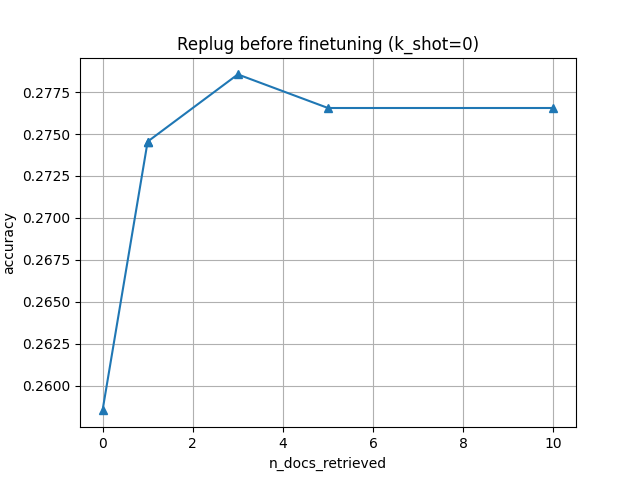
\includegraphics[width=0.8\linewidth]{figures/replug_before_finetuning.png}
    \caption{accuracy vs number of retrieved passages, replug inference strategy}
    \label{fig:mmlu_passages}
\end{figure}

\section{Conclusion}
We developed, fine-tuned, and benchmarked a lightweight Retrieval-Augmented Generation (RAG) 
system for STEM domain discussions, curating all aspects of the database creation,
training and evaluation process. To showcase our system, we created a Streamlit web application
that allows to chat with our model in real-time, using RAG to retrieve from Wikipedia as well as from
provided Arxiv papers.

From our experiments, we found that even a very small LLM significantly benefit from retrieval, and that, 
surprisingly, with such a small model concatenating all retrieved passages is more effective than averaging
next token probabilities over conditioning documents. We also found that the k-shot setting is detrimental to
performance with such a small model. [Comment on accuracy during training]

\newpage

\bibliography{wiki-savvy-rag}
\bibliographystyle{acl_natbib}
\nocite{*}

\appendix

\section{Appendix}
\label{sec:appendix}

\subsection{Faiss indexes}

\begin{figure}[h]
    \centering
    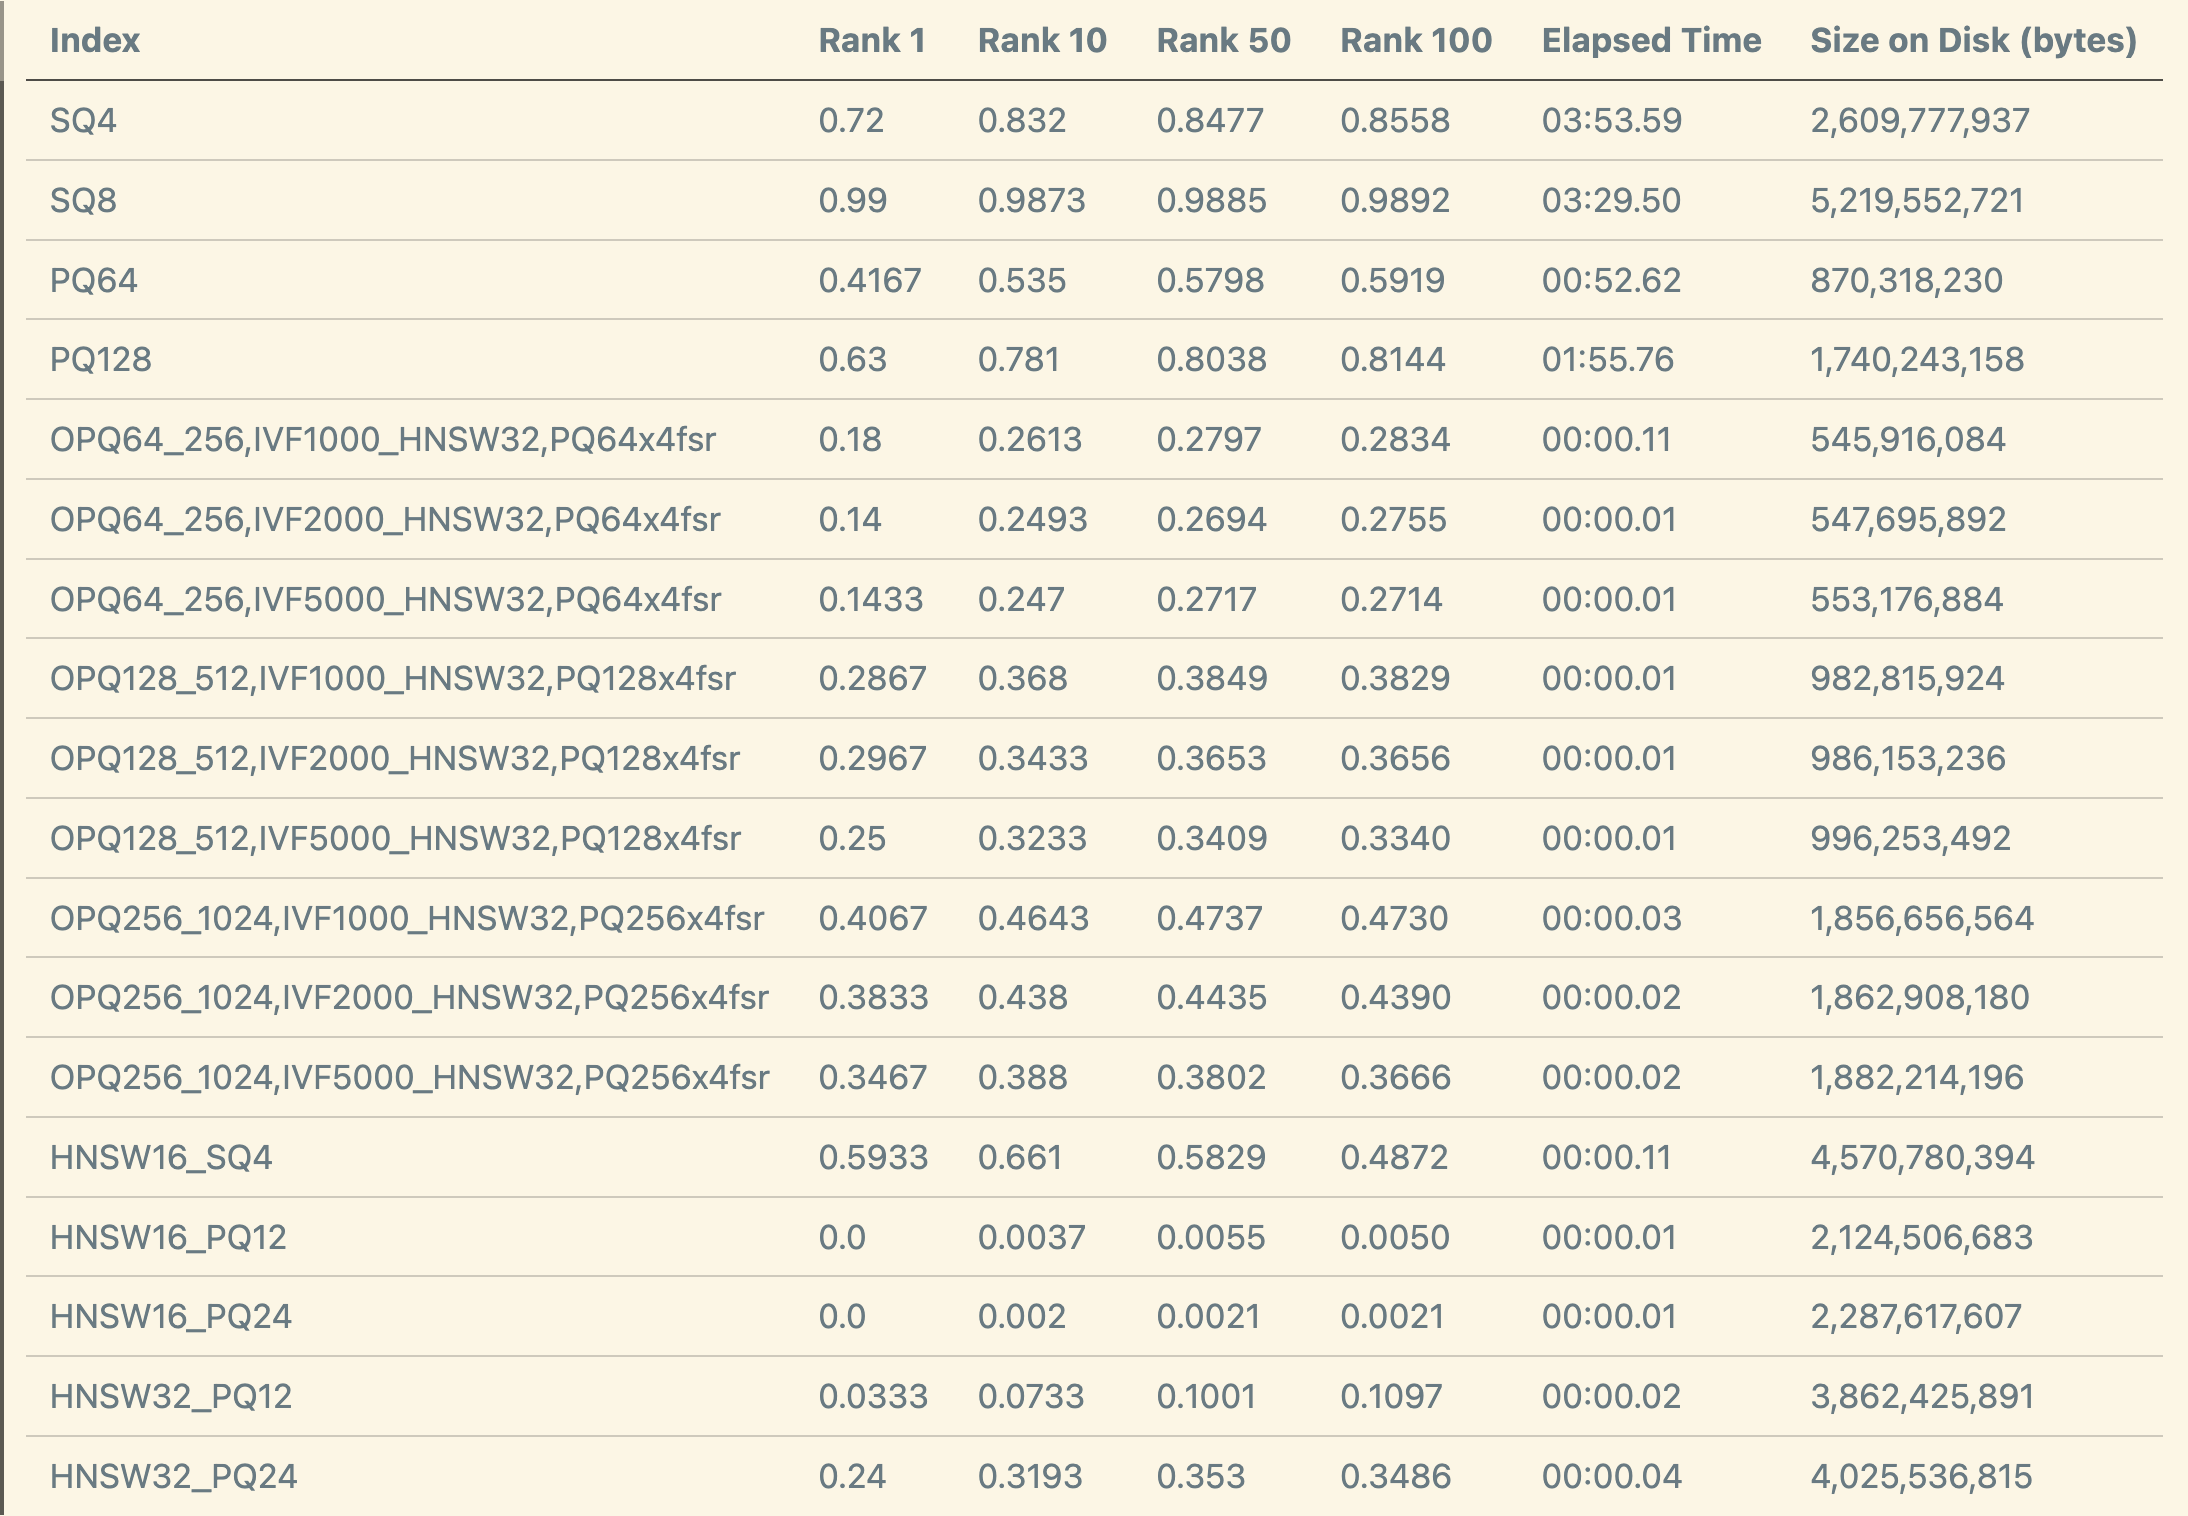
\includegraphics[width=0.8\linewidth]{figures/faiss-indexes-extensive.png}
    \caption{Extensive comparison of Faiss indexes. Rank n is the top-n recall using exhaustive search as ground truth.}
    \label{fig:faiss-indexes-extensive}
\end{figure}

\subsection{Training plots}

\sideBySideImages{figures/paramsA.png}{figures/paramsB.png}{0.48}{fig:params}{Evolution of the histogram of the parameters during training. left: A adapter of a self attention layer. right: B adapter of a mlp layer}

\sideBySideImages{figures/gradientsA.png}{figures/gradientsB.png}{0.48}{fig:gradients}{Evolution of the histogram of the gradients during training. left: A adapter of a self attention layer. right: B adapter of a mlp layer}

\subsection{Other ablations on MMLU}

\begin{figure}[h]
    \centering
    \includegraphics[width=0.8\linewidth]{figures/k_shots_ablation.png}
    \caption{we compare the different number of examples (shots) given to
    the model in the prompt}
    \label{fig:mmlu_shots}
\end{figure}

\begin{figure}[h]
    \centering
    \includegraphics[width=0.8\linewidth]{figures/k_shots_ablation.png}
    \caption{we compare the different number of examples (shots) given to
    the model in the prompt}
    \label{fig:mmlu_shots}
\end{figure}

In \ref{fig:mmlu_strategies} we compare the different inference strategies (naive and REPLUG).

\subsection{Checkpoints comparison on MMLU}

In \ref{fig:checkpoints} we compare the performances of different model checkpoints on the MMLU dataset.

\end{document}
